%%=============================================================================
%% Methodologie
%%=============================================================================

\chapter{\IfLanguageName{dutch}{Methodologie}{Methodology}}
\label{ch:methodologie}

%% TODO: Hoe ben je te werk gegaan? Verdeel je onderzoek in grote fasen, en
%% licht in elke fase toe welke stappen je gevolgd hebt. Verantwoord waarom je
%% op deze manier te werk gegaan bent. Je moet kunnen aantonen dat je de best
%% mogelijke manier toegepast hebt om een antwoord te vinden op de
%% onderzoeksvraag.
\section{Scenario 1: alledaags gebruik}
\lipsum[1-4]

\section{Scenario 2: professioneel IT-gebruik}
\lipsum[1-4]

\pagebreak
\section{Proof-of-concept Swift applicatie}
Het opzet van deze \textit{proof-of-concept} applicatie is het creëren van een applicatie die uitvoerbaar is op zowel iOS als macOS en dat met een minimum aan overtollige code of verlies aan performantie. Deze opstelling is mogelijk sinds 2020 dankzij de transitie van Intel x86 processoren naar de \textit{Apple Silicon} ARM architectuur \autocite{Apple2020}. Het is tevens belangrijk om te vermelden dat deze platformonafhankelijke manier van applicatie-ontwikkeling enkel mogelijk is op Mac toestellen die gebruik maken van een \textit{Apple Silicon} processor, zijnde de M1, M1 Pro, M1 Max of de M1 Ultra \autocite{AppleDeveloper2022a}. Indien u wenst te controleren of uw toestel gebruik maakt van een \textit{Apple Silicon} processor, dan kan u dit doen via het “Over deze Mac” dialoogvenster. Omwille van privacyredenen is het serienummer in de onderstaande afbeelding onleesbaar gemaakt.

\begin{figure}[h]
    \centering
    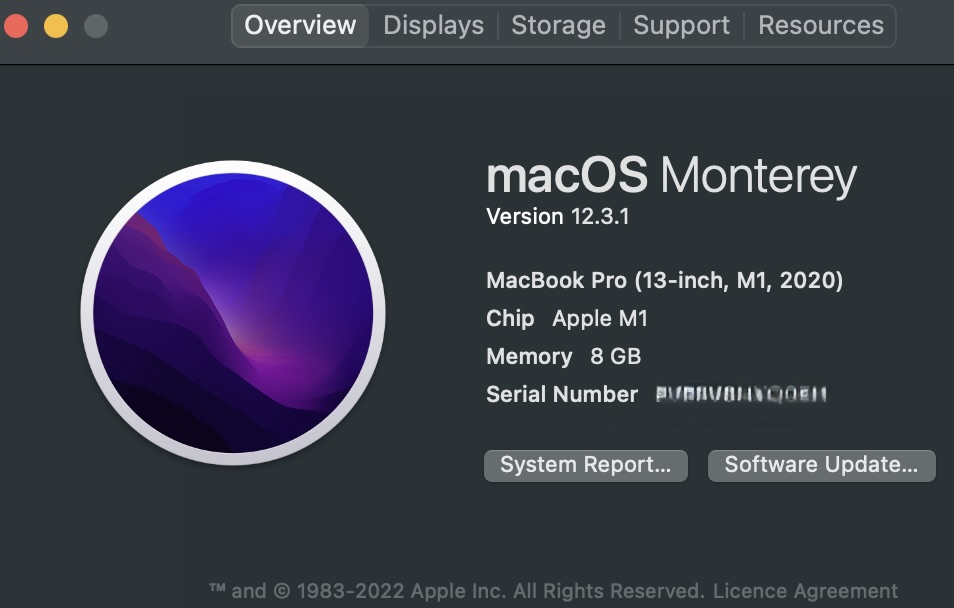
\includegraphics[width=100mm, scale=0.5]{img/overdezemac.jpeg}
    \caption{Het macOS 'Over deze Mac dialoogvenster'}
\end{figure}

De Swift programmeertaal is ontwikkeld door Apple en is reeds in gebruik sinds 2014. Deze wordt gebruikt voor het maken van \textit{native} applicaties voor iOS, iPadOS, macOS, tvOS en watchOS \autocite{AppleDeveloper2022b}. \textit{Native} applicaties worden gecompileerd in de machinetaal van het gekozen hardwareplatform. Vandaar dat applicaties die zijn ontwikkeld voor x86 toestellen niet uitvoerbaar zijn op het ARM platform en vice versa \autocite{Gillis2022}. De Swift taal combineert vaak gebruikte elementen uit de C, Objective C en Python programmeertalen en wordt gekenmerkt door eenvoud en performantie. Er wordt algemeen aangenomen dat Swift applicaties eenvoudiger te ontwikkelen zijn dan hun C en Kotlin tegenhangers omwille van de beginners- en gebruiksvriendelijke syntaxis \autocite{AppleDeveloper2022b}.

Apple voorziet uitstekende handleidingen voor zowel beginners als gevorderden, deze zijn tevens gratis verkrijgbaar in de \textit{Apple Books} online boekenwinkel. Verder stelt Apple een rudimentaire \textit{integrated development environment} (IDE) ter beschikking genaamd Swift Playgrounds. Deze is gericht op beginnende programmeurs of kinderen en jongeren die voor het eerst in aanraking komen met software ontwikkeling. Swift Playgrounds is gratis te verkrijgen op het iPadOS en macOS platform \autocite{AppleDeveloper2022b}.

Xcode is de IDE bij uitstek voor Swift ontwikkelaars aangezien deze een goede balans levert tussen nuttige functies en gebruiksgemak. De bijhorende simulator stelt ontwikkelaars in staat om hun applicaties meteen te testen in een gevirtualiseerde omgeving. Ondersteuning voor de \textit{Apple Silicon} architectuur is inbegrepen in Xcode sinds versie 12. Dit onderzoek maakt gebruik van Xcode 13.3.1 en de bijhorende toepassingen \autocite{AppleDeveloper2022a}.

De \textit{proof-of-concept} applicatie omvat een eenvoudige \textit{hard-coded} nieuwsapplicatie, dit houdt in dat de app niet kan bijgewerkt  worden zonder aanpassingen te maken aan de broncode. Verder maakt de app ook geen gebruik van \textit{API calls}. De focus van dit onderzoek ligt namelijk op het onderzoeken van de compatibiliteit en het gebruiksgemak van de applicatie op meerdere platformen en niet op het ontwikkelen van een geavanceerd programma dat gericht is op consumentengebruik.

Vooraleer men aanvangt met een project is het aangewezen om te controleren of het besturingssysteem en de IDE gebruikmaken van de meest recente softwareversies. In het geval van macOS is dit uitvoering 12.3.1 en bij Xcode is dit versie 13.3.1.

\begin{figure}[!h]
    \centering
    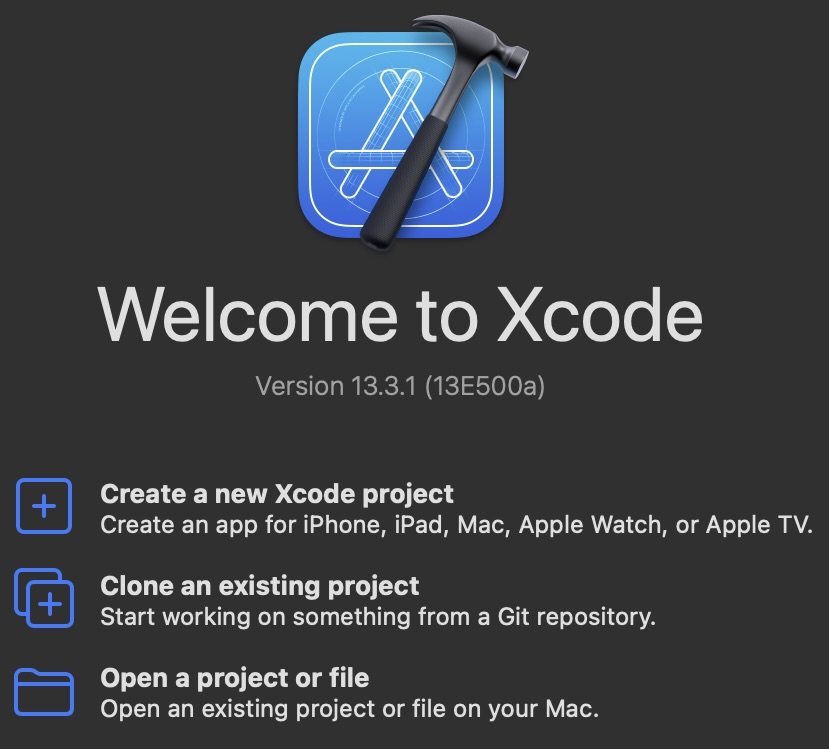
\includegraphics[width=90mm, scale=0.7]{img/xcodeversie.jpeg}
    \caption{Het startscherm van Xcode 13}
\end{figure}

Om te starten met de ontwikkeling van een nieuwe applicatie volstaat het om te kiezen voor de “Create a new Xcode project” optie. Vervolgens verschijnt er een dialoogvenster waar u kan kiezen tussen verschillende sjablonen gaande van iOS applicaties tot programma’s die gericht zijn op het tvOS platform. In het kader van dit onderzoek volstaan de “multiplatform” en “other” sjablonen. Gezien het doel van dit onderzoek, namelijk het onderzoeken van een “multiplatform“ applicatie is, is het aangewezen om te kiezen voor het “other” sjabloon aangezien deze de ontwikkelaar additionele flexibiliteit biedt.

\begin{figure}[!h]
    \centering
    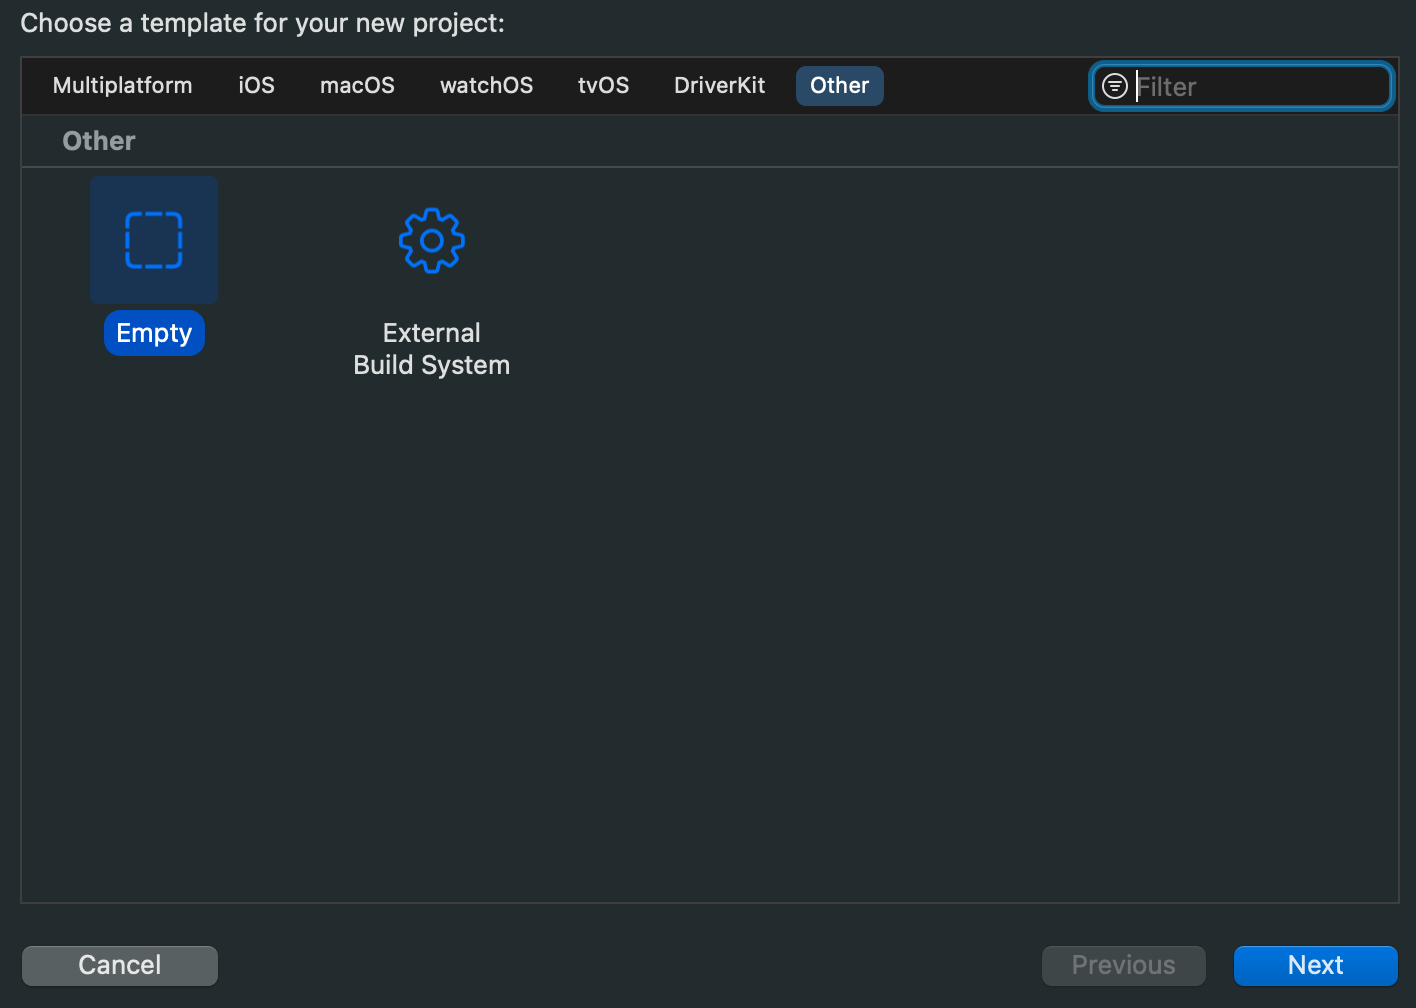
\includegraphics[width=110mm, scale=0.7]{img/otherproject.png}
    \caption{Xcode 13 sjablonen}
\end{figure}

\pagebreak
Na het kiezen van een sjabloon dient een ontwikkelaar een \textit{target} toe te voegen. Een \textit{target} specificeert een te bouwen product en bevat de instructies om dit product te bouwen vanuit een set bestanden in een project- of werkruimte. Een \textit{target} definieert één enkel product, het organiseert de invoer in het bouwsysteem, de bronbestanden en tenslotte de instructies voor het verwerken van de bronbestanden die nodig zijn om het product te bouwen \autocite{AppleDeveloper2011}. Een project kan één of meerdere \textit{targets} bevatten, in het geval van dit project zijn dit macOS en iOS.
\begin{figure}[!h]
    \centering
    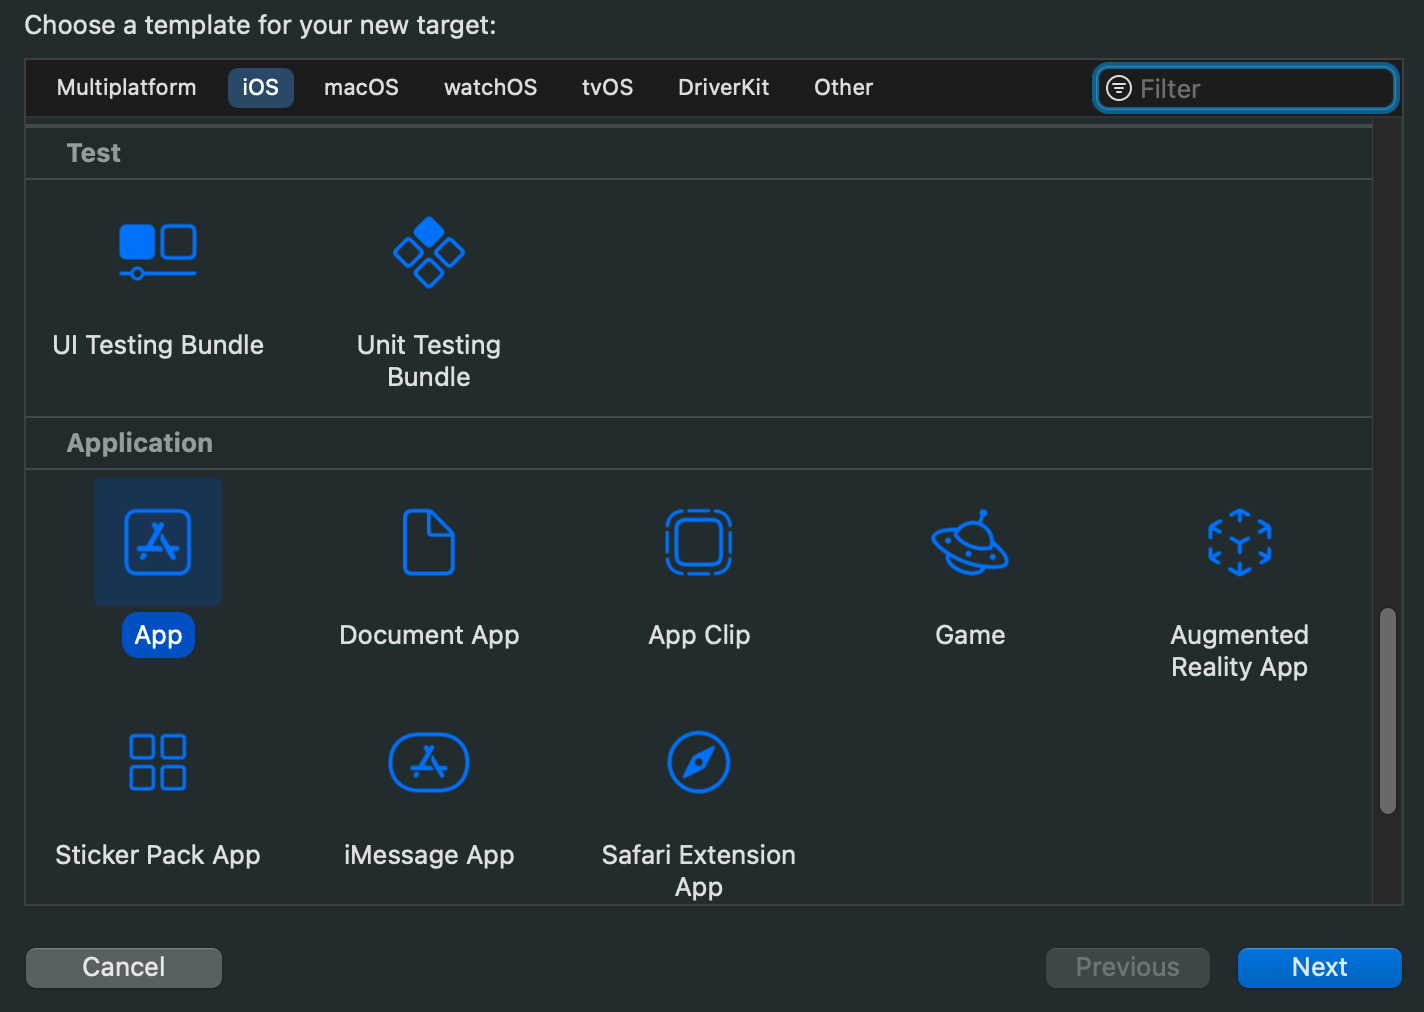
\includegraphics[width=110mm, scale=0.7]{img/iostarget.png}
    \caption{Een overzicht van de verschillende targets}
\end{figure}

\begin{figure}[!h]
    \centering
    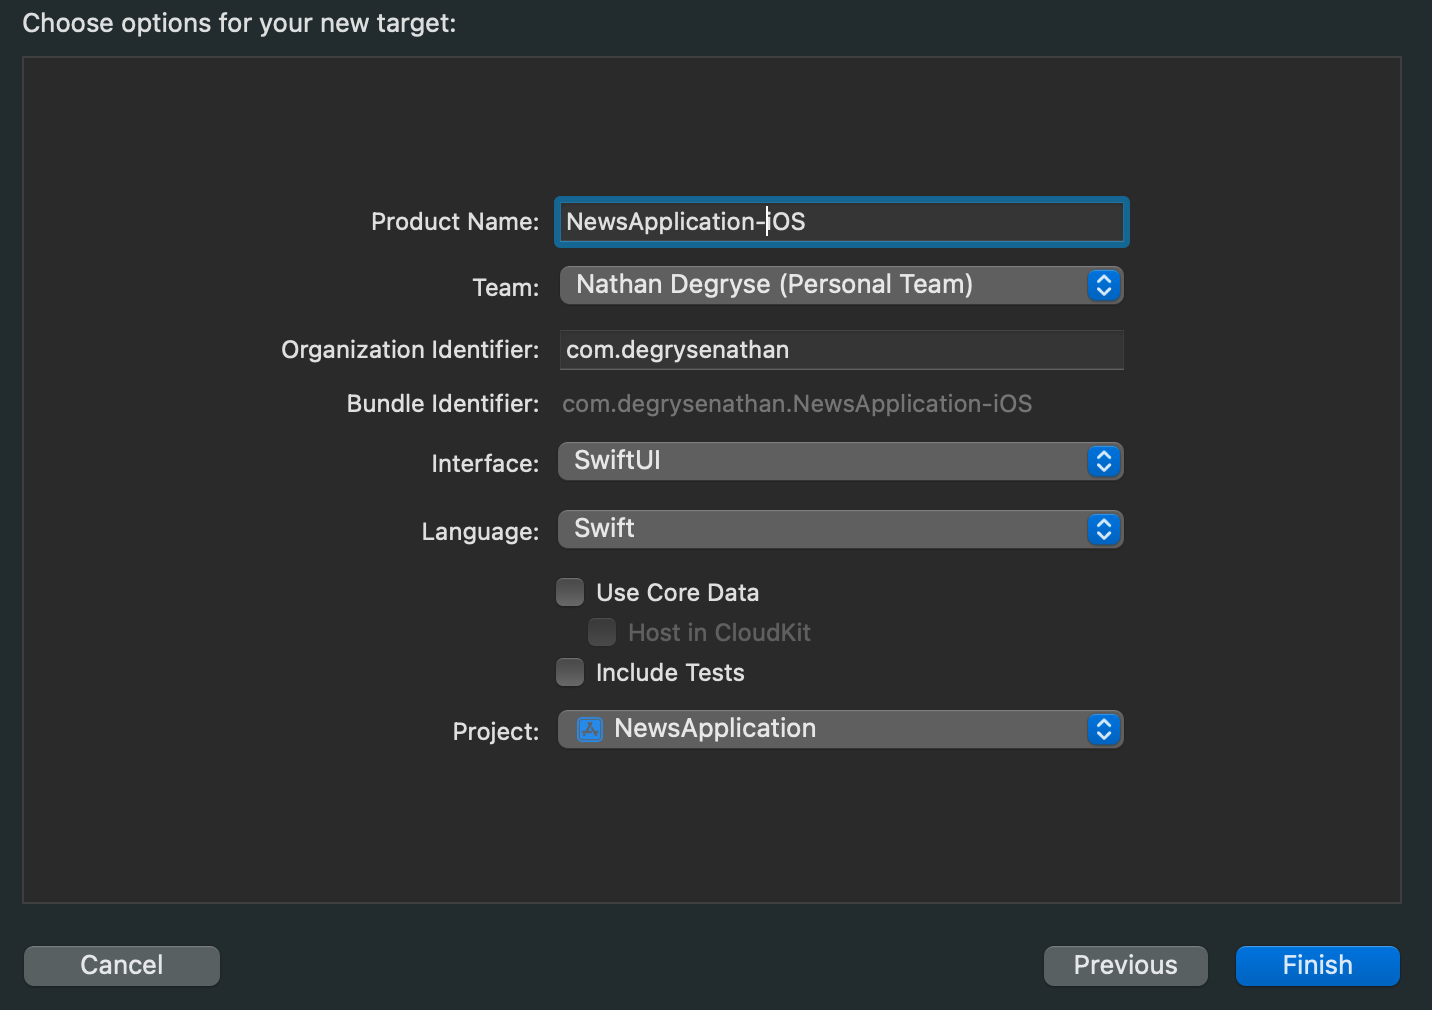
\includegraphics[width=120mm, scale=0.7]{img/iostargetdetail.png}
    \caption{Een detailweergave van het iOS target}
\end{figure}

\newpage
Eenmaal de iOS en macOS \textit{targets} zijn toegevoegd aan het project, is het tijd om een gedeelde \textit{group} aan te maken die in dit geval de naam “shared” heeft gekregen. In deze gedeelde \textit{group} zullen alle \textit{models} en \textit{views} worden opgeslagen. Deze zijn allen toegankelijk vanuit de iOS en macOS targets. De \textit{shared group} kan vervolgens uitgebreid worden met de \textit{models group} waar alle Swift \textit{structures} terechtkomen. \textit{Structures} zijn gelijkaardig aan klassen in andere programmeertalen, maar toch zijn er enkele opmerkelijke verschillen. Een klasse is een \textit{reference type} terwijl een \textit{struct} een \textit{value type} is. Wanneer men een \textit{struct} kopieert, krijgt men twee unieke kopieën van de gegevens. Echter wanneer men een klasse kopieert, verkrijgt men twee verwijzingen naar één instantie van de gegevens \autocite{Khan2021}. De \textit{Article struct} is als volgt opgebouwd: 

\begin{figure}[!h]
    \centering
    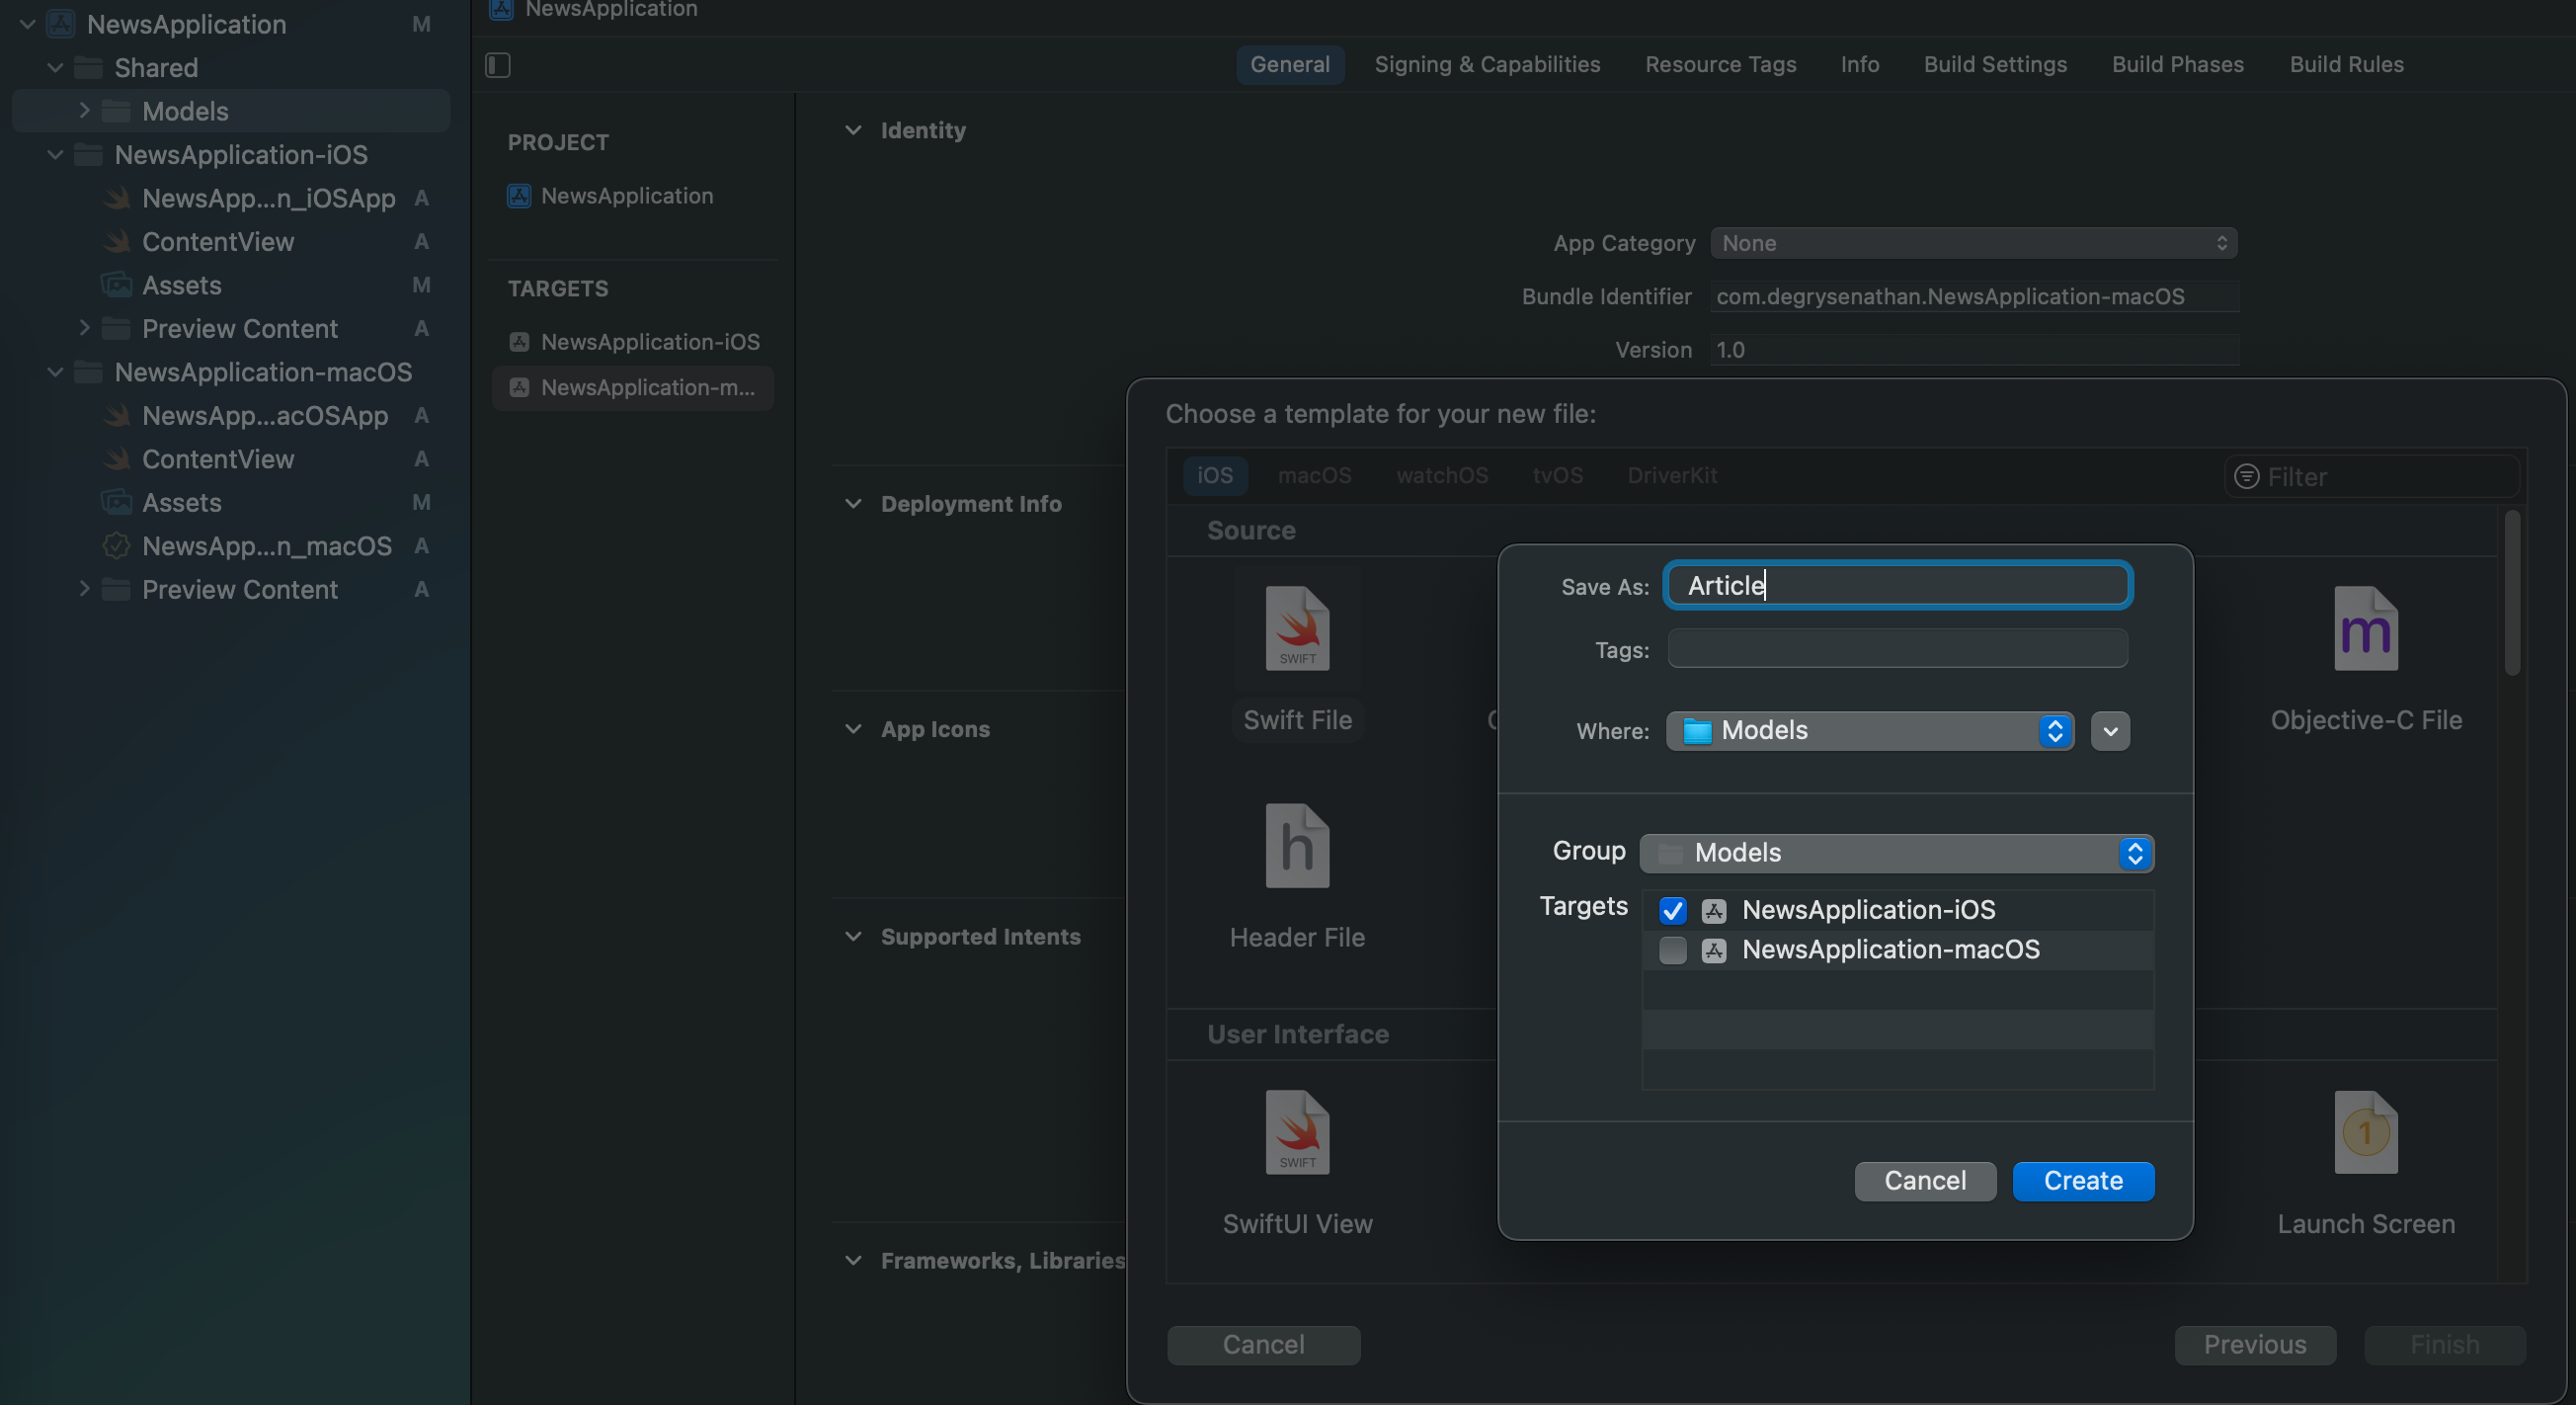
\includegraphics[width=120mm, scale=0.7]{img/articleswift.png}
    \caption{Een overzicht van het initialisatievenster van Article.swift}
\end{figure}

\newpage
\begin{lstlisting}
    
    //  Article.swift
    //  NewsApplication-iOS
    //
    //  Created by Nathan Degryse on 11/05/2022.
    
    import Foundation
    
    enum Subject: String {
        case all = "All"
        case sport = "Sport"
        case internationaal = "Internationaal"
        case regionaal = "Regionaal"
        case politiek = "Politiek"
    }
    
    extension Subject {
        
        var title: String {
            switch self {
                case .all:
                return "All"
                case .sport:
                return "Sport"
                case .internationaal:
                return "Internationaal"
                case .regionaal:
                return "Regionaal"
                case .politiek:
                return "Politiek"
            }
        }
        
    }
    
    struct Article: Identifiable{
        let id = UUID()
        let name: String
        let photo: String
        let description: String
        let rating: Int?
        let subject: Subject
    }
    
\end{lstlisting}
\newpage

Naast de \textit{models group} komt ook de group met alle preview content in de shared group terecht. Apple verwacht dat developers gebruikmaken van SwiftUI \textit{previews}, dit zijn voorvertoningen die live worden bijgewerkt wanneer een ontwikkelaar nieuwe elementen toevoegt of bestaande elementen aanpast/verwijdert. U kunt de standaard asset-catalogus "Preview Assets" gebruiken om voorbeeldafbeeldingen, kleuren en andere soorten assets te configureren die u normaal aan een asset-catalogus zou toevoegen. In dit project wordt de asset-catalogus gebruikt om een voorvertoning te genereren van de afbeeldingen die aan bod zullen komen in de nieuwsartikelen \autocite{VanDerLee2021}. Het is essentieel om aan te geven dat de "Preview Assets" beschikbaar zijn voor beide targets aangezien deze beide gebruik zullen maken van de afbeeldingen.

\begin{figure}[!h]
    \centering
    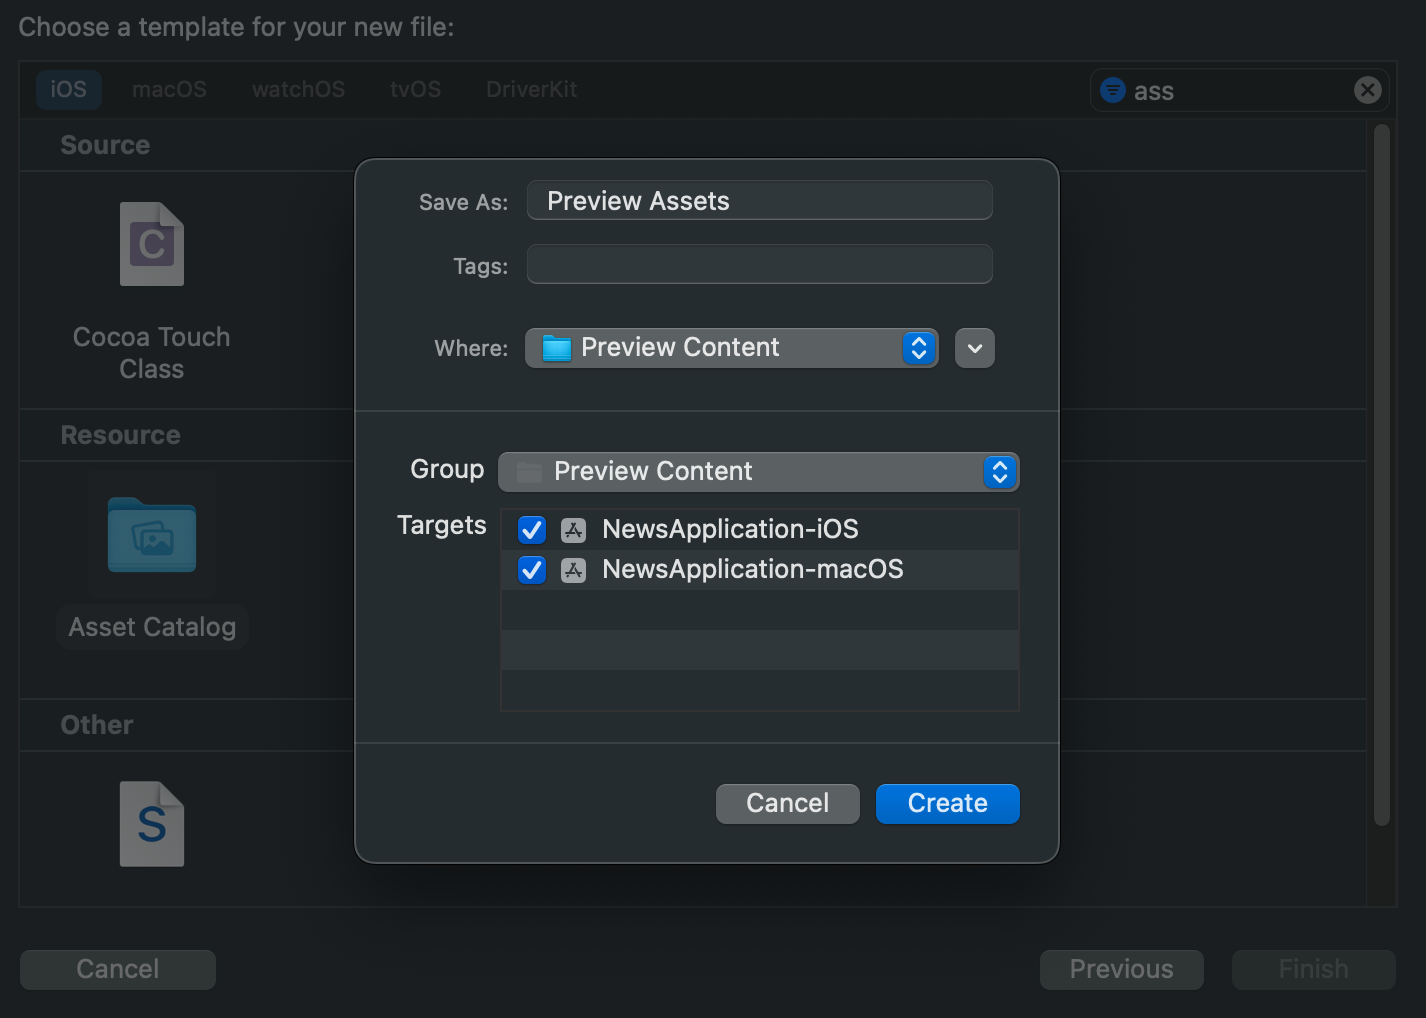
\includegraphics[width=\linewidth]{img/previewassets.png}
    \caption{Een overzicht van het initialisatievenster van de preview assets}
\end{figure}

\pagebreak 
In deze fase van het project is het cruciaal om de \textit{target membership} van de Article.swift file te verifiëren of aan te passen. Deze dient namelijk beschikbaar te zijn voor zowel het iOS- als macOS \textit{target} aangezien beide applicaties gebruik zullen maken van dit bestand.

\begin{figure}[!h]
    \centering
    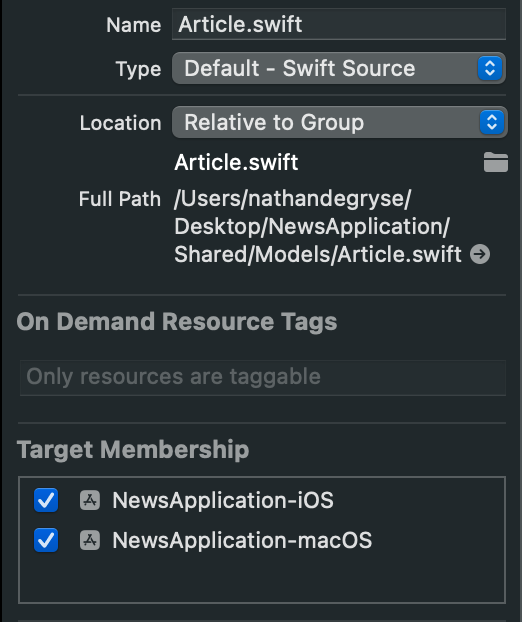
\includegraphics[width=80mm, scale=0.5]{img/articletargetmembership.png}
    \caption{Een overzicht van het targetmembership}
\end{figure}

Tenslotte dient de \textit{views group} ook toegevoegd te worden aan de \textit{shared group}. Deze \textit{group} bestaat uit de volgende \textit{views} die gedeeld moeten worden tussen de verschillende \textit{targets}:

\begin{itemize}
    \item \textbf{ArticleListView:} Deze \textit{view} zal gebruikt worden om een lijstvoorstelling te genereren op basis van alle beschikbare nieuwsartikelen. Deze lijst neemt het volledige scherm in beslag op de iOS applicatie, maar neemt echter slechts een deel van het scherm in beslag op de macOS applicatie. Dit omwille van de extra schermruimte die ter beschikking is op grotere toestellen zoals laptops en desktops.
    \item \textbf{ArticleDetailView:} Deze \textit{view} wordt gebruikt om een detailweergave voor te stellen van het desbetreffende artikel. Op het iOS platform neemt dit het volledige scherm in beslag terwijl dit op het Mac platform slechts een deel confisqueert. 
    \item \textbf{RatingView:} Tenslotte zal deze \textit{view} een grafische voorstelling weergeven van de recensie van het betreffende artikel. 
\end{itemize}

Het is opnieuw essentieel om beide \textit{targets} toe te voegen aan alle \textit{views}.

\pagebreak
Eenmaal alle \textit{views} zijn geïmplementeerd in de gedeelde \textit{group} dient men te refereren naar deze vanuit de \textit{target} producten zijnde de iOS en macOS applicaties. In onderstaande afbeelding is te zien hoe dit wordt verwezenlijkt in Swift. Via een \textit{navigation view} kan een gebruiker navigeren doorheen een verzameling binnen een navigatie-gebaseerde applicatie. Gebruikers navigeren naar een weergave door middel van een \textit{NavigationLink} te selecteren die de ontwikkelaar verstrekt. Op iPadOS en macOS verschijnt de inhoud van de bestemming in de volgende beschikbare kolom. Op andere platformen zoals iOS en watchOS wordt een nieuwe weergave op de stapel geplaatst en kunnen items uit de stapel worden verwijderd met platform specifieke besturingselementen, zoals een terug-knop of een veegbeweging \autocite{AppleDeveloper2022c}.

\begin{figure}[!h]
    \centering
    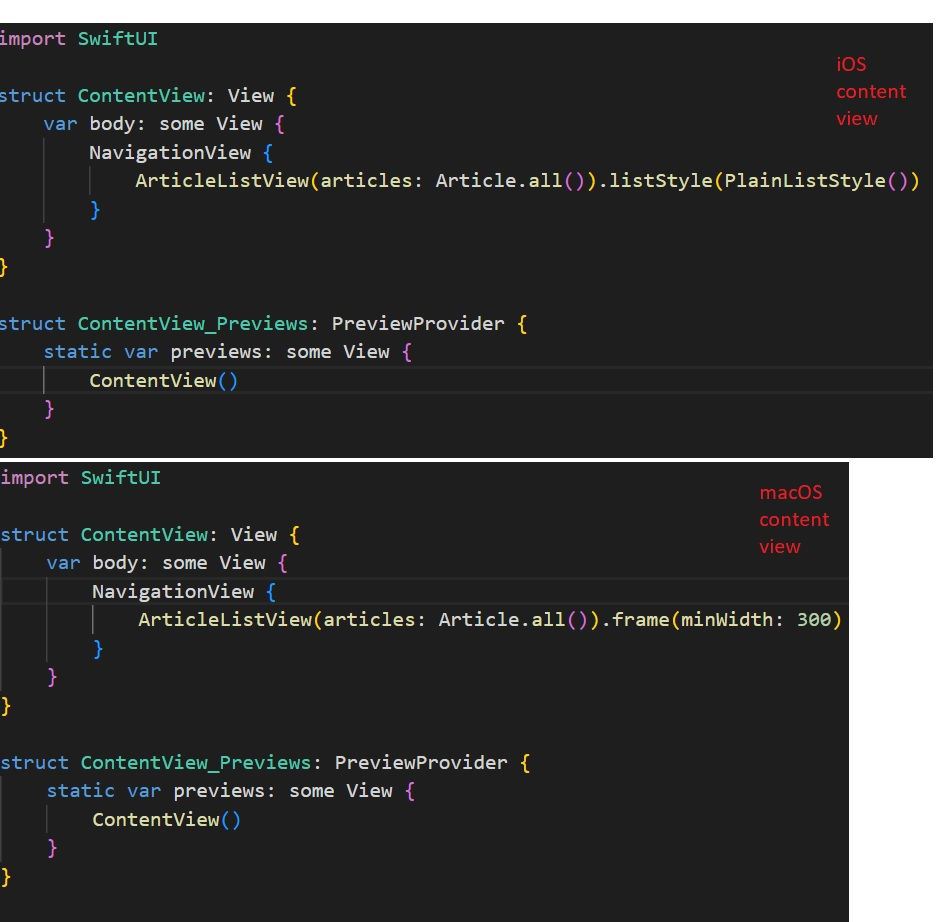
\includegraphics[width=\linewidth]{img/contentview.jpg}
    \caption{Een weergave van de ContentView files}
\end{figure}

\pagebreak
In de onderstaande afbeelding is er tenslotte een overzicht beschikbaar van de finale programmastructuur. Deze omvat de iOS en macOS nieuwsapplicaties die gebruikmaken van de gedeelde \textit{views}, \textit{models} en \textit{preview assets}.

\begin{figure}[!h]
    \centering
    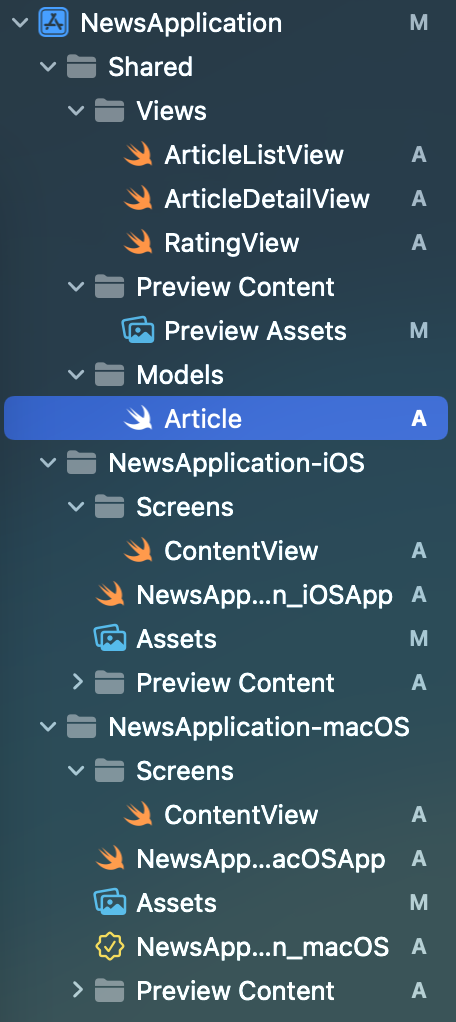
\includegraphics[width=70mm, scale=0.7]{img/applicatiestructuur.png}
    \caption{Een systematisch overzicht van de applicatiestructuur}
\end{figure}

\pagebreak
Deze finale afbeelding biedt een weergave van de iOS en macOS applicaties die simultaan uitvoerbaar zijn. Deze maken gebruik van simulatiesoftware die een onderdeel is van Xcode 13. Nadat een ontwikkelaar een applicatie heeft ontwikkeld, kan deze gecompileerd worden en kan men deze uitvoeren op een gesimuleerd of een echt apparaat. Een voordeel van de gesimuleerde aanpak is dat men de ontwikkelde applicatie kan testen op een uitgebreid gamma van virtuele apparaten gaande van de iPod Touch tot de meest recente iPhone modellen \autocite{AppleDeveloper2021}. De volledige broncode van dit project is beschikbaar via onderstaande URL: \url{https://github.com/DegryseNathan/ARM-van-mobile-naar-desktop/tree/main/NewsApplication}
\\\\
\begin{figure}[!h]
    \centering
    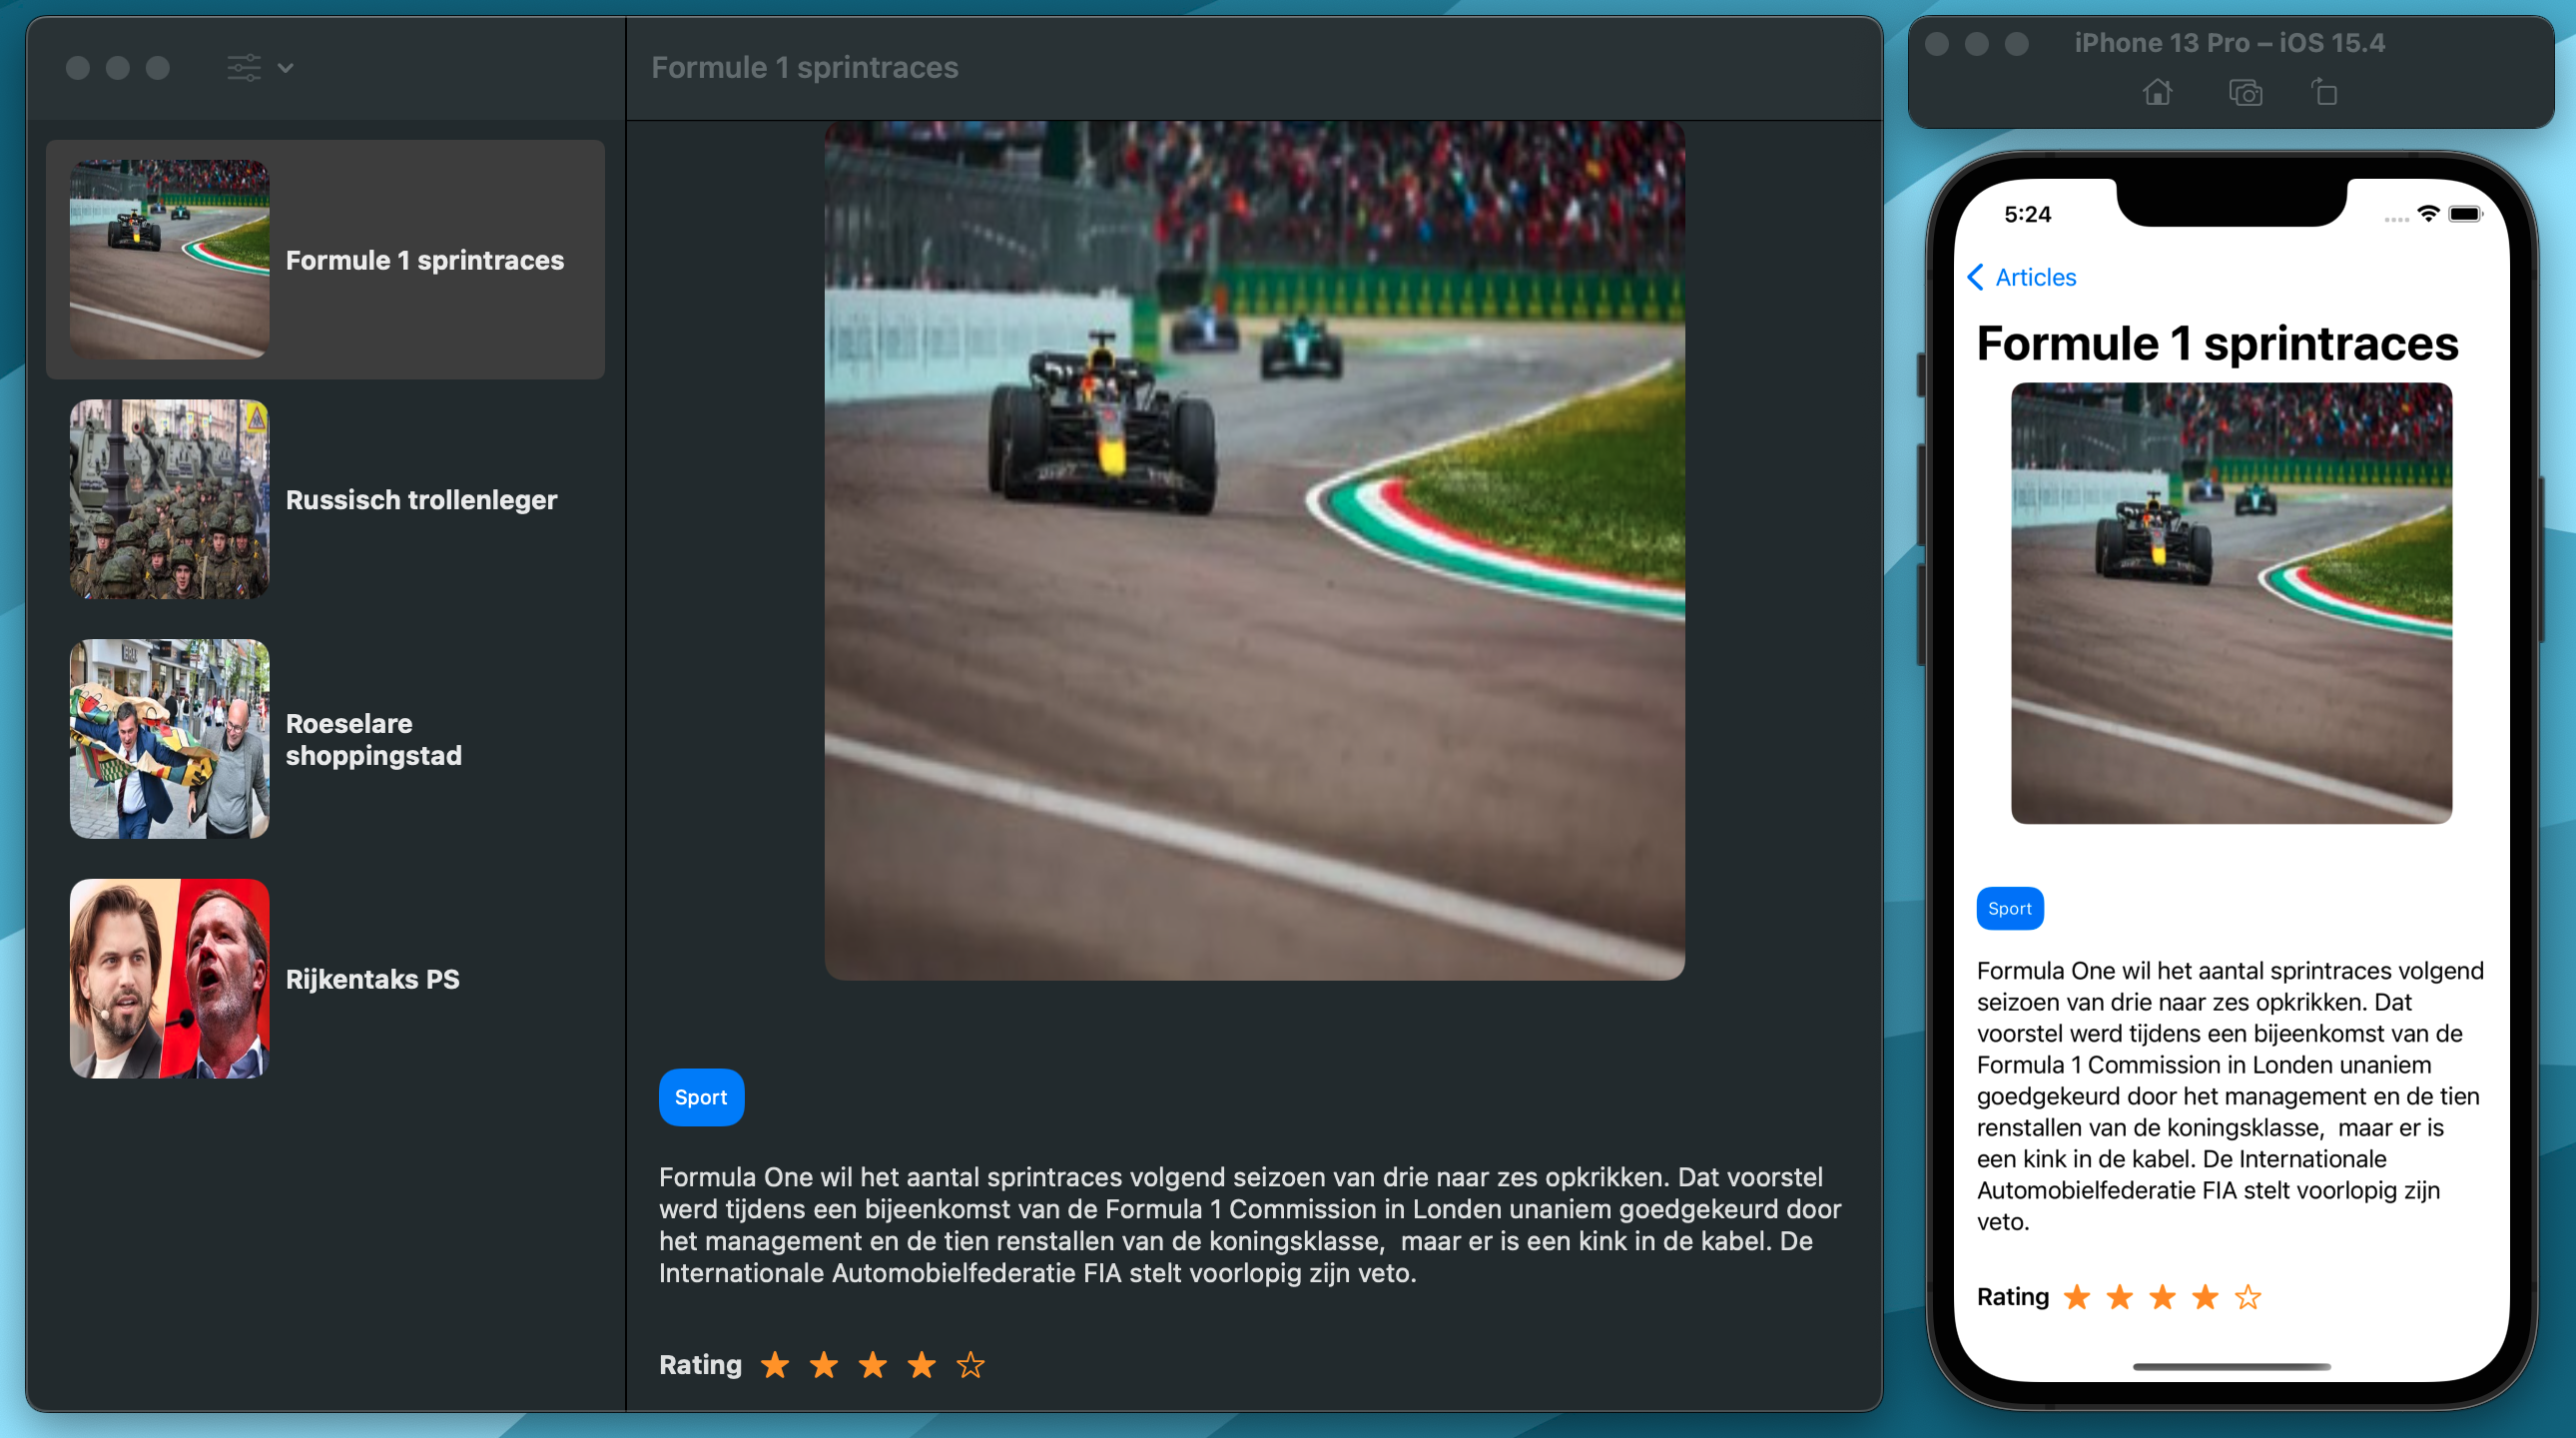
\includegraphics[width=\linewidth]{img/iosenmacosapplicatie.png}
    \caption{Een overzicht van de iOS en macOS nieuwsapplicatie}
\end{figure}
